\documentclass[12pt, oneside]{amsart}
\usepackage[margin=1in]{geometry}
\geometry{letterpaper}
\usepackage[parfill]{parskip}
\usepackage{url}
\usepackage{graphicx}

\title{Distributed Meta-Analysis for the Global Climate Prospectus}
\author{James Rising, Solomon Hsiang}

\begin{document}

\section{Background}

The Distributed Meta-Analysis System (DMAS) played a central role in the America's Climate Prospectus research, beyond its original purpose of collecting and combining econometric results.  The DMAS software was extended to perform the calculations to apply these results to weather data and aggregate the impacts, perform a number of specific analyses such as for return-period and adaptation, and distribute the load for these computations across cloud computing resources.

At a minimum, these same processes will be needed for the Global Climate Prospectus.  This proposal describes each of these functions, and how it will need to be scaled-up for the GCP.  Further, in the course of producing the ACP, there was a lot of learning about how to produce results efficiently, identify problems, and check intermediate steps.  This proposal includes several improvements, to ensure that the process is smoother in the GCP.

The general approaches to ensuring accuracy in the GCP fall into four areas.  First, the connection between documentation in the technical appendices, in internal wikis, and within the code and within the output files will be solidified, both through organizational and software methods (see section \ref{sec:betterdocs}).  Second, more of the design of the computations will be exposed, and transparently available to team members who are not otherwise involved in the development of DMAS (see section \ref{sec:functiongen}).  Third, conventions across all teams\footnote{Described in \url{https://docs.google.com/document/d/1TPxclzoakbB0M-wxtCRP62i8Uqk-kw8Dh2LkxDneYjU/edit}} will be used to automatically flag potential problems (see sections \ref{sec:versioncheck} and \ref{sec:unitchecks}).  Fourth, the development of new computations will include writing ``unit tests'': fully encapsulated diagnostics, which can all be processed repeatedly to ensure that new changes never break existing calculations (see section \ref{sec:unittest}).

{\it Throughout this proposal, time estimates are given as full-time DMAS developer times.  New developers who need to learn the system should double the time requirements.}

{\bf Bold-faced notes are requirements for people outside of the DMAS team, when interacting with the DMAS team.}

\section{Additional Research Scientists}

Three additional positions are described below.  The two research scientists are positions are intended as Ph.D. student RAships or half-time post-doctoral positions for one year.  If Ph.D. students, they would ideally be based at Columbia.

{\bf Environmental Economist 1 - Historical Lead}

This position requires a research scientist familiar with Python and econometrics.  He or she will have the following responsibilities:

\begin{itemize}
\item Constructing a collection of impact models, monitoring their computation, handling and evaluating results, and documenting all related material.
\item Constructing diagnostics for these and other impact models and analyses.
\item Handling baseline data files (manipulating the files and writing associated Python to work with the data) (see section \ref{sec:baselines}).
\item Generating historical and no-climate-change impact runs (see section \ref{sec:historical}).
\item Generating return-time calculations and analyses (see section \ref{sec:returntime}).
\item Developing the logic which applies different models in different regions (see section \ref{sec:globalcombo}).
\item Consolidate results into tables (quantiles and Excel sheets) for further analysis or display (see section \ref{sec:tables}).
\end{itemize}

{\bf Environmental Economist 2 - Futures Lead}

This position requires a research scientist familiar with Python and econometrics.  He or she will have the following responsibilities:

\begin{itemize}
\item Constructing a collection of impact models, monitoring their computation, handling and evaluating results, and documenting all related material.
\item Constructing diagnostics for these and other impact models and analyses.
\item Managing the logic that produces aggregations and analyses based on aggregations (see section \ref{sec:aggregation}).
\item Expanding the adaptation logic to be able to be applied in all cases, based on input from the internal IAM (see section \ref{sec:adaptation})
\item Produce the sources of variation analyses and displays (see section \ref{sec:variations})
\item Developing the communication between the Internal IAM and the computation processes (see section \ref{sec:internaliam})
\item Developing the external API for communication with external IAMs (see section \ref{sec:externaliam})
\end{itemize}

{\bf Scientific Software Developer}

This position requires a software developer familiar with Python, web development, and scientific computing.  He or she will have the following responsibilities:

\begin{itemize}
\item Developing the cloud computation monitoring and execution dashboard (see section \ref{sec:dashboard}).
\item Constructing the expression-builder tool interface (see section \ref{sec:functiongen}).
\item Developing the logic to apply expressions built in the expression-builder tool to future weather data (see section \ref{sec:evaluation}).
\item Developing the logic to estimate expressions built in the expression-builder tool given historical data (see section \ref{sec:estimation}).
\item Developing visualization and interaction features for communicating GCP results (see section \ref{sec:visualinteract}).
\end{itemize}

\section{Ensuring Accuracy}

\subsection{Better Documentation}
\label{sec:betterdocs}

Redundancy within the documentation is important, to ensure that the relevant documentation is available in every location it is needed.  However, this redundancy threatens to allow documentation in different locations to be inconsistent.  This section describes how to ensure that it is not.

Documentation will be available in five locations:
\begin{description}
\item[The Internal Wiki (\url{https://bitbucket.org/ClimateImpactLab/meta/wiki/Home})] This contains both technical documentation (e.g., calculation definitions), and organizational documentation (e.g., who is responsible for what).
\item[Technical Appendices] This contains technical documentation appropriate for public consumption.
\item[The DMAS Website] Annotations defined in the website will describe the functions, units (see section \ref{sec:unitchecks}), and calculations (see section \ref{sec:functiongen}).
\item[Code Comments] This will often be more finely grained than the technical appendices, but will also include high-level descriptions appropriate for the technical appendices.
\item[Input and Output Files] The common header in the input and output files will include basic information on the units (see section \ref{sec:unitchecks}) and calculations (see section \ref{sec:functiongen}).
\end{description}

This proposal specifies a ``master'' source for the documentation of all materials that use DMAS, and how the information there will be distributed to the other locations.

The master source for impact functions will be the DMAS Website, where the functions and calculations will be input.  A daily program will generate Markdown files, for the Internal Wiki, and \LaTeX\ files, for the Technical Appendices, by filling out a uniform template.  DMAS will also create the file headers to include units and calculations.

The master source for public-facing calculation details will be the code, through docstrings.  Only the docstring section {\tt Published:} will be included in the wiki and appendices.  The format of the comments is reStructuredText, backwards compatible to Markdown and including links to pages in the wiki.

{\it The Markdown and \LaTeX\ translation will require 1 week, including everything above.}

\subsection{Version Checks}
\label{sec:versioncheck}

The version system is designed to be checkable by simply searching the
text of code and data files, but an automated version checking system
can identify anything that falls through the cracks.  The version
checking system will encode the rules of version dependencies: that
calculations may only use inputs files that specify the same version
or a version contained in their dependencies.

{\it The version checking system will take .25 weeks to construct.}

{\bf Version information will be required for all input files.}

\subsection{Unit Checks}
\label{sec:unitchecks}

Units are specified in input and output files, and in impact
functions.  Units must always conform between these.  Various
calculations can convert units, and do so in computable ways.

The unit checking system will ensure that input units conform, and
that output units are included in files and as inputs to other
functions.  The system requires three components: a text parser and
formatter, to translate between textual representations of units; a
unit conversion system, which describes how multiplication changes
units; and a unit equivalence system, which describes how different
units are related through scaling constants.

{\it The unit checking system will be based on James's code in
  OpenWorld, and will take .5 weeks to translate and apply to DMAS.}

{\bf Unit information will be required for all input files and impact function definitions.}

\subsection{Unit Tests}
\label{sec:unittest}

Unit Tests are repeatable diagnostics, which check both the low-level
functioning of operations or high-level features of their results.
The DMAS team will use the PyUnit framework to perform unit tests at
both these scales.  The full suite of unit tests will be run at will
and regularly to ensure that every aspect of the system is working as
expected.

{\it Encapsulating the existing diagnostics into unit tests will take 1 week.}

{\bf Impact functions and new desired outputs from the DMAS system should be communicated with a description of unit tests that can be used to ensure that they are functioning properly.}

\section{Analysis Details}

\subsection{Baselines}
\label{sec:baselines}

Baseline data, which is used in DMAS for aggregation and
absolute-change results, will often need to be combined from several
datasets or inferred from population densities to provide sufficient
resolution.  In some cases, data will be provided by the authors of
impact function estimates.

For every baseline, a distinct set of assumptions will need to be
made, but the outlines will be similar.  The IPUMS database and other
global, high-resolution databases will be used to generate baselines
wherever possible.  These will be checked against country-level data,
such as UNSTATS or WorldBank, and adjusted to ensure consistency.
Then high-resolution population data, from LandScan, will be used to
infer country-consistent data where additional data is not available.

This process will be encoded in a repeatable mechanism, so that new
consistent files can be reproduced when IPUMS updates or if we need to
change our assumptions.

Finally, a master database of region-hierarchy baseline files will be
maintained in Bitbucket, using the standardized header.

{\bf When new socioeconomic baselines are required by any team, they
  should be added to the master database and advertised across the
  project.}

{\it The system to download and analyze IPUMS data, and use it,
  LandScan, and country-level data to generate consistent datasets,
  will require 1 week to construct.  Once it is ready, additional
  datasets will require .25 - .5 weeks to create each.}

\subsection{Global Combinations}
\label{sec:globalcombo}

Each impact (mortality and morbidity, energy costs, crime, etc.) will be described by several different empirically estimated functions within different regions.  In some regions, multiple impact estimates are available, while other regions will be outside of the domain of all existing studies.  The functional form used by different estimates may also differ.

Conceptually, a mapping will exist for each impact which describes for each locality a list of estimates to be used in computing results.  See section \ref{sec:appmapgen} for details on how this mapping will be generated.  Where different functional forms are used, the methods described in the extended Bayesian merging document\footnote{Available at \url{https://drive.google.com/drive/u/0/#folders/0BwjYswM_266ESDhvYkpNRmdWTEE/0BwjYswM_266EUXlDbDhVenN5Qms}} will be applied.

{\it Constructing the logic for generating and using mappings will take .25 - .5 weeks, and the extension to the Bayesian combination system will take 1 week.}

{\bf The zone of applicability for impact functions and fitting data need to be included with these materials.}

\subsection{Historical and No-Climate-Change Analyses}
\label{sec:historical}

Historical results apply impact functions to observed historical data,
while no-climate-change results produce a new century by reproducing
years of historical data and apply impact functions to these.

This system does not need changes from the ACP; however, the
Historical Lead needs to run it and prepare the results.

\subsection{Return-Time Calculations}
\label{sec:returntime}

Return-time results identify the 1-in-20 year threshold, using GCM
model results for the historical period, and then identify each time
this threshold is exceeded in the future runs, across the distribution
of Monte Carlo results.

This system does not need changes from the ACP; however, the
Historical Lead needs to run it and prepare the results.

\subsection{Consolidated Tables}
\label{sec:tables}

The impact results are provided in the form of ``every quantile''
files, for each region, 20-year period, and scenario.  In addition,
impact tables reformat the results across regions and scenarios, to
display select quantiles in Excel spreadsheets.

This system does not need changes from the ACP; however, the
Historical Lead needs to run it and prepare the results.

\subsection{Region Aggregation}
\label{sec:aggregation}

Impact results are computed at the highest available resolution, and
then aggregated to larger regions using baseline weights.

This system does not need changes from the ACP; however, the Futures
Lead needs to produce unit tests and manage the logic for it.

\subsection{Adaptation}
\label{sec:adaptation}

In the ACP, adaptation runs were separate analyses, where climatic
averages were used with region-specific estimates to adjust
coefficients over time.  In the GCP, this process will be extended.

First, socioeconomic variables will be used to condition the
adaptation process, and these will be generated for each region by the
internal IAM.  So, the system needs to be extended to handle
additional variables and a wider dimensionality of adaptation, and to
receive these variables from a new source (described in section
\ref{sec:internaliam}).

Second, adaptation will become more pervasive.  Although no-adaptation
runs will need to be generated, most impacts will allow for some form
of adaptation by default.  This will require more information for each
impact.

{\it Socioeconomic conditioning will require .25 weeks, and making it easier to run adaptation runs and separating them from no-adaptation runs will take another .25 weeks.}

\subsection{Sources of Variation}
\label{sec:variations}

The sources of variation analyses identify the variance across runs
that vary models, realizations, and impact functions while keeping the
others constant.  This requires ``median'' runs, as well as a system
to analyze the results.

This system does not need changes from the ACP; however, the Futures
Lead needs to produce unit tests and manage the logic for it.

\section{New DMAS Processes}

\subsection{Internal IAM Interaction}
\label{sec:internaliam}

An internal IAM will extend the CGE from the ACP (QED).  Rather than
considering impact results as exogenous to the IAM, impact results
will rely on IAM variables both as normal inputs and for conditioning
adaptation.  This requires a communication channel between DMAS and
the IAM.

The communication will use HTTP requests, so that the IAM and DMAS can
be running on different computers as needed.  The IAM will drive the
interaction, requesting each year while passing in a region-hierarchy
file of relevant variables (consisting of about 50 kB per variable).
DMAS will respond with a region-hierarchy file of impacts in that
year.  Direct port connections can be used for faster communication
when possible.

{\it The HTTP/Port communication system, along with logic for storing
  intermediate results between calls, will take 1 week to build.}

\subsection{External IAM Interaction}
\label{sec:externaliam}

External IAMs will have an interest in using the impact results from
DMAS.  The same basic system as for Internal IAM communication will be
used, with some additions.  First, individual impacts or intermediate
calculations for those impacts will be available using different (API)
calls.  These functions need to be built and documented on a public
page.  Second, external IAMs may require different assumptions and
settings, and these need to be maintained in user-specific accounts.

{\it The broader API will require 1 week to build and document.  The
  user/IAM settings will require .5 weeks to set up, or more depending
  on the extensiveness of those additional settings.}

{\bf The Futures Lead should be involved in focus groups with the IAM
  teams to ensure that they have what they need.}

\subsection{Monitoring and Execution Dashboard}
\label{sec:dashboard}

A number of tools were developed to execute computations in the cloud
computing environment of the ACP, monitor their progress, and collect
the results.  The dashboard is intended to allow this to happen
without executing terminal commands.  When new results are needed,
clicking a button on the dashboard will start them, and the dashboard
will show their progress, and the results will be downloadable from
the dashboard when they are ready.

This will be used both for generating the GCP and making the time
constraints transparent, and for allowing future users to generate
their own results in a managed environment.

{\it The dashboard will require 2 weeks to build and populate with the
  basic operations of the GCP.}

\subsection{Generating Functions}
\label{sec:functiongen}

Intuitively, the process of translating daily weather into yearly impacts using estimated impact functions can be very simple.  However, to handle the wide range of cases for doing that, the DMAS processing system is fairly complicated, including many possible functions and a level of abstraction than requires some experience.  However, these complications support a relatively simple ``top-level'' coding structure.  Users can define new calculations using existing functions.

This proposal takes this process a further step, by constructing a user-interface for defining calculations.  This serves three functions: making it easier to make and review calculations without knowing python; automatically generating documentation for the functions; and allowing the function definitions to be re-used for the purpose of estimating new impacts from data.

A mockup of the user-interface is shown below.

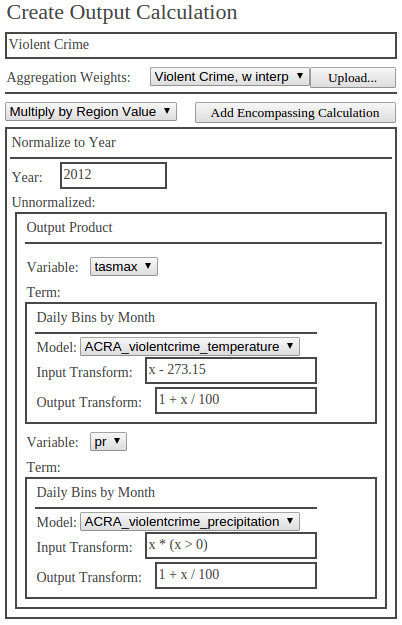
\includegraphics[width=4in]{wireframe.png}

This shows the calculations for violent crime.  The top section specifies just the calculation name and aggregation weights.  The section below is organized into nested boxes.  Each box is an intermediate calculation, which can be reported on its own.  Additional calculations, which further refine the calculations shown, can be added with the ``Add Encompassing Calculation'' button (here shown ready to add a ``Multiply by Region Value'' calculation, used to translate from relative to scaled changes).  The calculation described takes the product of two impact functions (one for temperature and one for precipitation), and then normalizes it by the value in year 2012.

{\it Constructing the user-interface will take 1 week.}

\subsection{Evaluating Expression-Builder Functions}
\label{sec:evaluation}

While the logic for evaluating functions is unchanged from the ACP,
expressions will be defined in the expression-builder rather than in
code.  Each element defined in the user-interface will need to be
mapped to a function, which upon evaluation is called and its results
send to the appropriate place.

{\it The logic for connecting the expression-builder to the evaluation
  module will take .5 weeks.}

\subsection{Estimating New Functions}
\label{sec:estimation}

The expression-builder will also have all of the necessary information
for estimating impact functions from data.  This will require an
entirely new system, which generates Stata code from the
expression-builder (which is separately downloadable), executes it,
and incorporates the results back into DMAS.

{\it The .do file generator will take 1 week, for allowing data files
  to be uploaded and organized will be .5 weeks, and the logic for
  reading Stata coefficient files will take .5 weeks.}

\subsection{Visualizations and Interactions}
\label{sec:visualinteract}

One of the most powerful ways for these results to have an impact is
with high-quality visualizations and online interaction tools.  The
Computer Scientist will develop tools for interacting with our process
and results.  This includes maps, colored by impact and clickable for
more information; ways to navigate between different impacts and
between the impacts and the functions that were used to produce them;
and ways to try out different scenarios (particular weather events or
functional changes) and see the results.

{\it There is easily 5 weeks of visualizations that could be planned
  out for the GCP that come directly from DMAS.}

\section{Implementation Details}

\subsection{Applicability Mapping Generation}
\label{sec:appmapgen}

In general, the applicability regions for impact functions will be
described using the region hierarchy (see the Computing Conventions),
as a list of regions (e.g., ``Africa, Madagascar'').  This will be
translated into a list of applicable impacts for each high-resolution
region.  For example:

\begin{verbatim}
Algeria: 519fba8f8309fa3ff0a978dd, 51e4292e8309fa3079841e23
Madagascar: 51e4292e8309fa3079841e23
...
\end{verbatim}

\subsection{Storage Locations}

Processed data files (e.g., region-hierachy files) will be stored in
Bitbucket (Git), with most of the source files being stored on
Shackleton.  However, the location of the source files will not need
to be consistent, and the details will be recorded on the Wiki.

\end{document}
